\documentclass[UTF8]{ctexart}

\usepackage{graphicx}
\usepackage{amsmath}

\title{空间几何与向量代数笔记}
\author{JohnsonLee}
\date{\today}

\begin{document}
\begin{titlepage}
\maketitle
\tableofcontents
\end{titlepage}
\section{空间直角坐标系与向量代数}
\subsection{空间直角坐标系}
三个轴,八个卦限。
\subsection{向量及其线性运算}
\subsubsection{加减法与数乘}
众所周知,向量是可以加减的,坐标表示对应坐标进行加减
\subsubsection{点乘/内积}
点乘与角(包括直线与直线,面与面,直线与面)的相关性很大
\subsubsection{外积}
外积可以用如下的形式记忆:
\begin{figure}[h]
$$\vec a=(x_1,y_1,z_1),\vec b=(x_2,y_2,z_2)$$
$$
  \vec a \times \vec b = 
  \begin{vmatrix}
    \vec i & \vec j & \vec k \\
    x_1 & y_1 & z_1 \\
    x_2 & y_2 & z_2
  \end{vmatrix}
$$  
  \caption{外积行列式形式}
  \label{外积行列式形式}
\end{figure}

注意外积的结果仍是向量,其方向由右手定则可以得到,大小参考图\ref{外积行列式形式},同时,图\ref{外积行列式形式}的大小等于$\vec a,\vec b$构成的平行四边形的面积。

外积等于$0$时,两向量平行.
\subsubsection{向量在坐标轴上的投影}
    1. $A'B'=|AB|\cos \phi$

    2. 两个向量的和在轴上的投影等于两个向量轴上投影的和
    
    3. 向量与数的乘积在轴上的投影等于向量在该轴上的投影与数的乘积
\subsubsection{向量的坐标,数量积,向量积}
    \subparagraph{方向角}$\alpha,\beta,\gamma$,对应非零向量分别与$x,y,z$轴构成的夹角
    $a_x = |\vec\alpha|\cos\alpha$;$y,z$轴以此类推

    有方向角有什么用呢?

    向量单位化。我们得到一个这样的向量$(\cos\alpha,\cos\beta,\cos\gamma)$,这个向量是原向量单位化的结果

    \subparagraph{柯西-施瓦茨不等式}
   $$\vec a\cdot\vec b \le |a|\cdot|b|$$   
   $$\sum_{i=1}^3 a_i\cdot b_i \le \sqrt{\sum_{i=1}^3 a_i^2\cdot\sum_{i=1}^3 b_i^2}$$
    \subparagraph{混合积}
    $$\vec a=(x_0,y_0,z_0),\vec b=(x_1,y_1,z_1),\vec c=(x_2,y_2,z_2)$$为三个不共线,不共面的向量,则三者会构成一个立方体,立方体的体积是几何?
    \begin{quote}
      立方体底面积:
      $$S=|\vec a \times \vec b|$$
      立方体的高:
      $$H = \vec c \cdot \frac{\vec a \times \vec b}{|\vec a \times \vec b|}$$
      立方体体积:
      $$V = S \cdot H = \vec c \cdot (\vec a \times \vec b)$$
      则知
      \begin{figure}[h]
      $$
        V = 
        \begin{vmatrix}
          x_0 & y_0 & z_0 \\
          x_1 & y_1 & z_1 \\
          x_2 & y_2 & z_2
        \end{vmatrix}
      $$  
        \caption{体积行列式形式}
        \label{体积行列式形式}
      \end{figure}
    \end{quote}
    当三个向量共面的时候,$V=0$即混合积为0
\section{平面、曲面、空间曲线及其图形}

\subsection{平面}
\subsubsection{平面方程}
\subparagraph{点法式方程}

  $M_0(x_0,y_0,z_0)$是平面上的一个已知点,$\vec n(A,B,C)$是平面的一个法向量,则平面的点法式方程可以表示为:
  $$A(x-x0) + B(y - y_0) + C(z - z_0) = 0$$

  若已知平面方程,平面的法向量怎么找呢?  
  
  看$x,y,z$前的系数不就可以了吗

\subparagraph{三点式方程}

  有了三个点,意味着我可以得到三个向量,而这三个向量共面,共面意味着混合积为0,则行列式为0.

  $A(x_1,y_1,z_1),B(x_2,y_2,z_2),C(x_3,y_3,z_3)$还有一个任意点$X(x,y,z)$

  $$\begin{vmatrix}x-x_1&y-y_1&z-z_1\\x_1-x_2&y_1-y_2&z_1-z_2\\x_2-x_3&y_2-y_3&z_2-z_3\end{vmatrix} = 0$$

  解出以上方程即可

\subparagraph{截距式方程}

  平面与$x,y,z$三轴分别交于$P(a,0,0),Q(0,b,0),R(0,0,c)$其中$a\ne0,b\ne0,c\ne0$易得平面的截距式方程为
  $$\frac{x}{a}+\frac{y}{b}+\frac{z}{c} = 1$$

\subsubsection{空间关系}
\subparagraph{两个平面之间的夹角}
两平面之间的夹角$\theta$(二面角)$\theta \in [0,{\pi \over 2}]$

如何求解夹角?
\begin{quote}
   求出两个平面的法向量,两向量之间的夹角为$\phi$,两平面之间的夹角为$\theta$,计算$\cos \phi,易证\phi = \theta$
\end{quote}

\subparagraph{两平面的位置特征}

\begin{quote}
$$\Pi_1 \perp \Pi_2 \Rightarrow A_1A_2 + B_1B_2 + C_1C_2 = 0$$
$$\Pi_1 \parallel \Pi_2 \Rightarrow {A_1 \over A_2}={B_1 \over B_2}={C_1 \over C_2}$$
\end{quote}

\subparagraph{点到平面距离}$$d=\frac{|Ax_0+BY_0+CZ_0+D|}{\sqrt{A^2+B^2+C^2}}$$
  怎么证明?

      我们已知平面的法向量为$\vec n =(A,B,C),x(x,y,z)$是平面内的一个点,得到一个向量是$\vec a = (x-x_0,y-y_0,z-z_0)$距离就是$\vec a$在法向量方向上的投影嘛
      $$d = \frac{|\vec n \cdot \vec a |}{|\vec n|} = \frac {|A(x-x_0) + B(y-y_0) + C(z-z_0)|}{\sqrt{A^2+B^2+C^2}}=\frac{|Ax_0+BY_0+CZ_0+D|} {\sqrt{A^2+B^2+C^2}}$$
\subparagraph{平行平面之间的距离}$$d=\frac{|D_1-D_2|}{\sqrt{A^2+B^2+C^2}}$$
  怎么证明?

  我们在两平面上分别任取一点$A(x_1,y_1,z_1),B(x_2,y_2,z_2)$,可以得到一个向量$\vec{AB}$,两平行的平面距离就等于$\vec {AB}$在法向量方向上的投影嘛。
  $$d = \frac{\vec {AB} \cdot \vec n}{|\vec n|} = \frac{|A(x_1-x_2)+B(y_1-y_2)+C(z_1-z_2)|}{\sqrt{A^2+B^2+C^2}} = \frac{|D_1-D_2|}{\sqrt{A^2 + B^2 + C^2}}$$
\emph{两直线之间的距离}

我们知道了平行平面之间的距离怎么求,能否利用两平面之间的距离等于两平面上的两异面直线之间的距离来求解直线之间的距离呢?

可以!

假设直线$L_1$的方向向量为$\vec n_1$,$L_2$的方向向量为$\vec n_2$,易得
$$\vec n_3 = \vec n_1 \times \vec n_2$$
$\vec n_3$垂直于$L_1,L_2$,而以$\vec n_3$为法向量,过$L_1$构成一个平面$\Pi_1$,以$\vec n_3$,过$L_2$构成一个平面$\Pi_2$。$\Pi_1,\Pi_2$是平行的,且$L_1$在$\Pi_1$内,$L_2$在$\Pi_2$内则$\Pi_1,\Pi_2$间的距离等于$L_1,L_2$间的距离。
\begin{figure}[ht]
  %\centering
  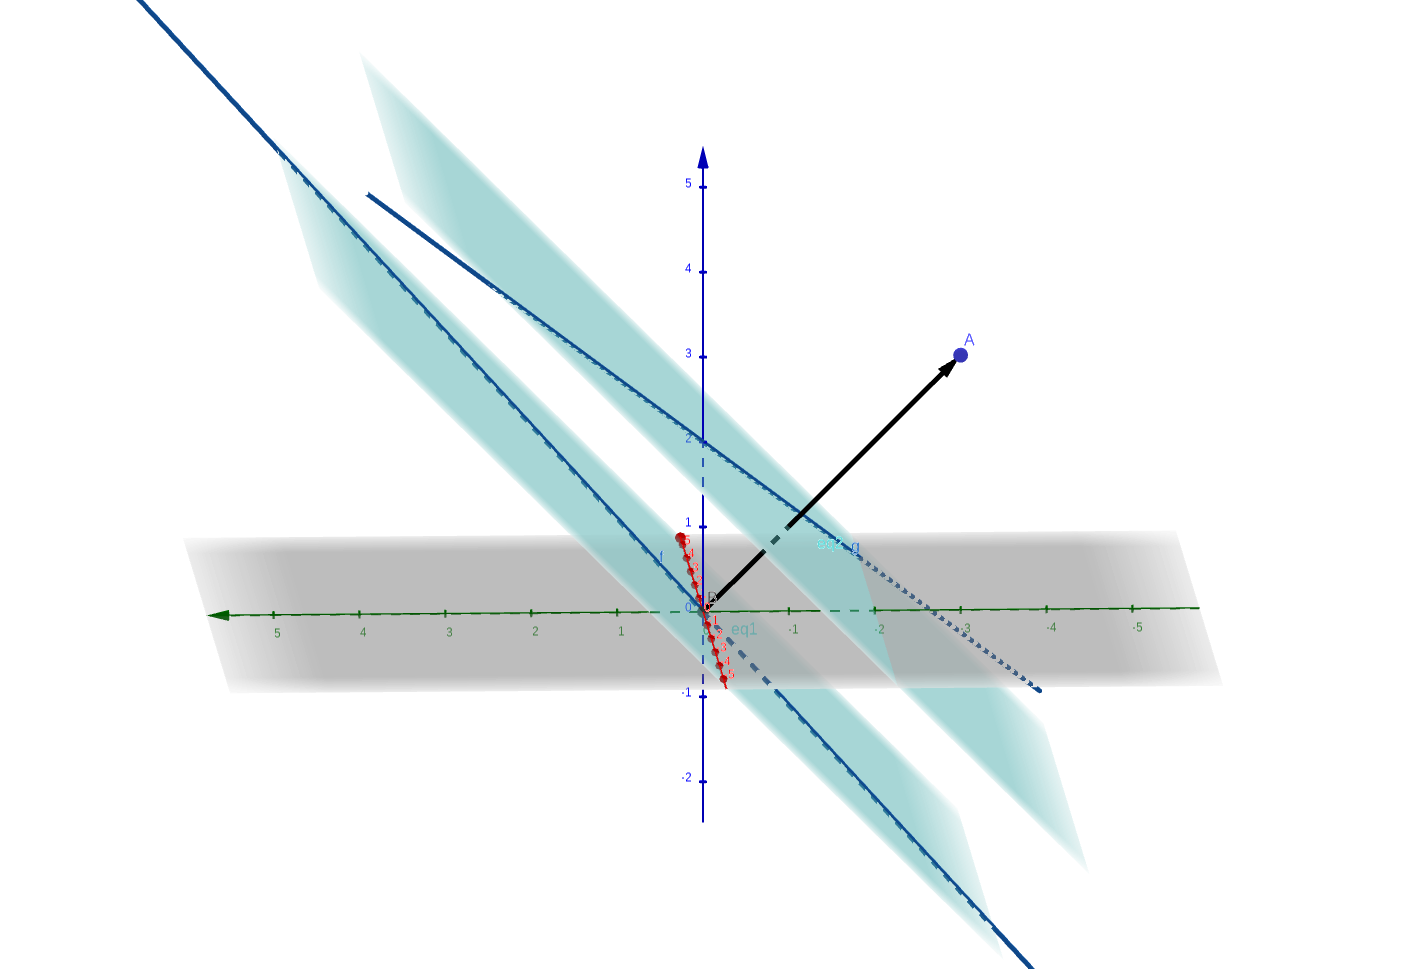
\includegraphics[width = 10cm]{../picturenote/直线之间距离示意图.png}
  \caption{直线之间距离示意图}
  \label{直线之间距离}
\end{figure}

\subsection{直线}

\subsubsection{方程}
   \subparagraph{一般方程}直线是两个平面的交线,则用两个平面方程联立来确定一条直线
   \subparagraph{两点式方程}推到点向式方程,因为两点可以得到一个向量$\vec l = (m,n,p)$
   \subparagraph{点向式方程}有一个平行于直线的向量$\vec l = (m,n,p)$则直线方程可以写作
   $$\frac{x-x_0}{m}=\frac{y-y_0}{n}=\frac{z-z_0}{p}$$
   \subparagraph{参数方程}同上已知方向向量,直线的参数方程可以写作:
   $$\begin{cases}  {x = x_0 + mt}\\{y = y_0 + nt}\\z = z_0 + pt\end{cases}$$

   \subparagraph{已知一般方程,怎么求直线方向向量?}
   分别得到两个平面的法向量以后,由于直线在两个平面内,则直线与两个法向量都垂直,也就是说方向与两法向量叉积结果相同。

\subsubsection{空间关系}
  \subparagraph{两直线夹角}即是两方向向量的夹角,范围在$(0,\frac \pi 2)$

  \subparagraph{两直线之间距离}参考图 \ref{直线之间距离}

  \subparagraph{两直线公垂线的求法}暗含在图 \ref{直线之间距离} 中了

\subsection{平面束}
\emph{平面束}:通过一条直线的全部平面组成的平面称为平面束
$$L:\lambda_1(A_1x+B_1y+C_1z+D_1=0) + \lambda_2(A_2x+B_2y+C_2z+D_2)=0 (\lambda_1 * \lambda_2 \ne 0)$$
注意平面束方程存在退化情况(两个平面重合)以及两个平面平行的特殊情况
实际使用时我们经常两边除以$\lambda_1$以简化方程,然而,在非退化情况下这样的方程不能表示出第二个平面,因此我们使用的时候要格外小心,注意讨论第二个平面是否符合条件.

\subsection{曲面和空间曲线}

曲面S满足一个三元方程 $F(x,y,z) = 0$,若看作集合则有:

$$S = \{(x,y,z)|F(x,y,z) = 0\}$$

则$F(x,y,z) = 0$是曲面$S$的方程。

\subsubsection{方程}

  \paragraph{一般方程}

    $$\begin{cases}F(x,y,z) = 0 \\G(x,y,z) = 0\end{cases}$$

  \paragraph{参数方程}

    \begin{figure}[ht]
      \centering
      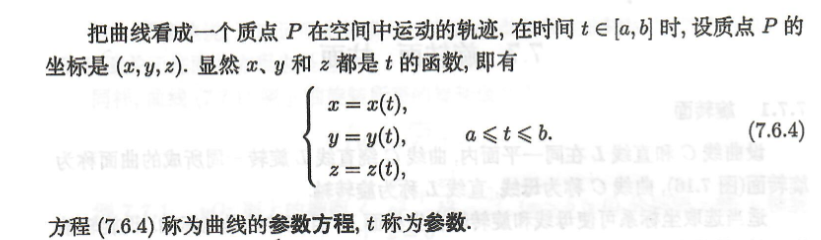
\includegraphics[width = 12cm]{../picturenote/参数方程.png}
      \caption{曲线的参数方程}
    \end{figure}


\subsubsection{旋转面、柱面}

\paragraph{旋转面}

既然是旋转面就一定有一条旋转轴,还有一条母线,用这两个东西肯定可以得到方程

  \begin{figure}[ht]
    \centering
    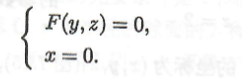
\includegraphics[width = 10cm]{../picturenote/旋转面参数方程.png}
    \caption{曲线的参数方程}
  \end{figure}

绕轴旋转意味着什么?见高等数学上p214

绕着谁旋转,则谁不变例如$F(y,\sqrt{x^2+z^2})$

\paragraph{旋转椭球面}

\subparagraph{方程}(其实都是由$F(\sqrt {x^2+y^2},z))$等公式推出的,绕谁转,谁不变,另外一元换,看哪两项可以凑出原来对应的平面曲线方程(母线方程)就知道了
$$\frac{x^2}{a^2}+\frac{y^2}{a^2}+\frac{z^2}{b^2} = 1$$
$$\frac{x^2}{b^2}+\frac{y^2}{a^2}+\frac{z^2}{a^2} = 1$$

\paragraph{旋转单叶双曲面,旋转双叶双曲面}
单叶双曲线就是以对称轴为轴进行旋转得到的,双叶双曲面是以双曲线两定点所连成直线为轴旋转而成的

通过方程看出是单叶还是双叶的方法

单叶:两正一负 双叶:两负一正

\paragraph{旋转抛物面}
一般都是绕对称轴旋转
\paragraph{柱面}
路径作为准线,过路径上一点,垂直与坐标轴的点成为直母线
方程之中少了哪一个字母就平行于哪一个轴(并不常常这样,因为有时候母线是斜的,就你妈邪门)

\subsubsection{重要曲面}

\paragraph{重要曲面1}

\subparagraph{球面}

$x^2 + y^2 + z^2 = R^2$

\subparagraph{圆锥面}
$x^2 + y^2 = z^2$(由$y = z$ 绕$z$轴旋转而来)

\subparagraph{旋转双曲面} 
$\frac{x^2}{a^2} + \frac{y^2}{b^2} - \frac{z^2}{c^2} = 1$

\paragraph{重要曲面2}

\subparagraph{圆柱面}
$x^2 + y^2 = R^2$

\subparagraph{抛物柱面}
$x^2 = 2py(p>0)$
\subparagraph{椭圆柱面}
$\frac{x^2}{a^2} + \frac{y^2}{b^2} = 1$

\paragraph{重要曲面3}

\subparagraph{椭球面}  
$$\frac{x^2}{a^2} + \frac{y^2}{b^2} + \frac{z^2}{c^2} = 1$$
\subparagraph{椭圆抛物面} 
$$\frac{x^2}{2p^2} + \frac{y^2}{2q^2} = z$$ (p,q同号)
\subparagraph{马鞍面}
\subparagraph{单叶双曲面}
\section{常见题型整理}

\end{document}

